\section{Experiments}
This section reports baseline results on three representative models and illustrates how MIRAGE-V exposes taxonomy-specific weaknesses.
All numbers in this section are computed from the released evaluation harness outputs (CSV summaries and per-example predictions).

\subsection{Setup}
We evaluate a MIRAGE-V suite of \NumExamples examples grouped into \NumModules modules (100 examples / 50 minimal pairs per module).
To enable apples-to-apples comparison across models with different native video interfaces, we use a \textbf{frame-based protocol}: each video is decoded into \textbf{\FramesPerVideo} uniformly sampled frames, and all models are prompted with the same sampled frames and a yes/no question.

\subsection{Models}
We evaluate:
\begin{itemize}[leftmargin=*]
  \item \textbf{GPT-5.2} (OpenAI API, frame inputs).
  \item \textbf{Gemini-2.5-Flash} (Gemini API, evaluated on the same sampled frames).
  \item \textbf{Qwen2.5-VL-7B} (open-weight, local inference via Hugging Face Transformers).
\end{itemize}
All models are instructed to answer \texttt{YES} or \texttt{NO} only (no explanation) to reduce parsing ambiguity.

\subsection{Aggregate performance}
Table~\ref{tab:overall} reports overall accuracy and pair accuracy.
GPT-5.2 achieves the highest individual-example accuracy (\BestAcc\%), while Gemini-2.5-Flash achieves the highest pair accuracy (\BestPairAcc\%).
However, pair accuracy remains below 28\% for all models, indicating that even when models answer single examples moderately well, they often fail to \emph{discriminate} minimally different clips.

\begin{table}[t]
  \centering
  \small
  \caption{Overall results on \NumExamples examples (\FramesPerVideo uniform frames per video). We bold the best score in each column.}
  \label{tab:overall}
  % Auto-generated from overall.csv
\begin{tabular}{lrrrr}
\toprule
Model & $N$ & Acc. (\%) & Pair Acc. (\%) \\
\midrule
GPT-5.2 & 1000 & \textbf{61.0} & 27.2 \\
Gemini-2.5-Flash & 1000 & 57.0 & \textbf{27.4} \\
Qwen2.5-VL-7B & 1000 & 53.5 & 20.8 \\
\bottomrule
\end{tabular}

\end{table}

\subsection{Accuracy by taxonomy module}
Figure~\ref{fig:by-module-accuracy} and Table~\ref{tab:by-module-accuracy} break down accuracy by taxonomy module.
We observe three consistent patterns:

\paragraph{(i) Near-chance accuracy hides shortcut behavior.}
Several modules cluster near 50\% accuracy (e.g., C-CHAIN, P-OCC, TM-ID, PH-INVAR-ENERGY).
Because MIRAGE-V pairs flip the correct answer between $A$ and $B$ by construction, a model that defaults to one answer can achieve $\approx$50\% accuracy while failing to detect the intervention.

\paragraph{(ii) Coarse temporal aggregation is easier than fine-grained physics checking.}
Counting (R-COUNT) is comparatively easy for all models, with near-perfect accuracy for GPT-5.2 and Qwen2.5-VL-7B.
Event ordering (TR-ORDER) is also relatively easier for Gemini and Qwen, while GPT-5.2 is near chance on this module under sparse sampling.

\paragraph{(iii) Latent-property inference remains challenging.}
Inferring mass and friction from dynamics (PH-LATENT-MASS / PH-LATENT-FRICTION) exposes clear gaps across models.
In particular, PH-LATENT-FRICTION is the hardest module on average, and Qwen2.5-VL-7B fails completely on this module in this evaluation protocol.

\begin{figure}[t]
  \centering
  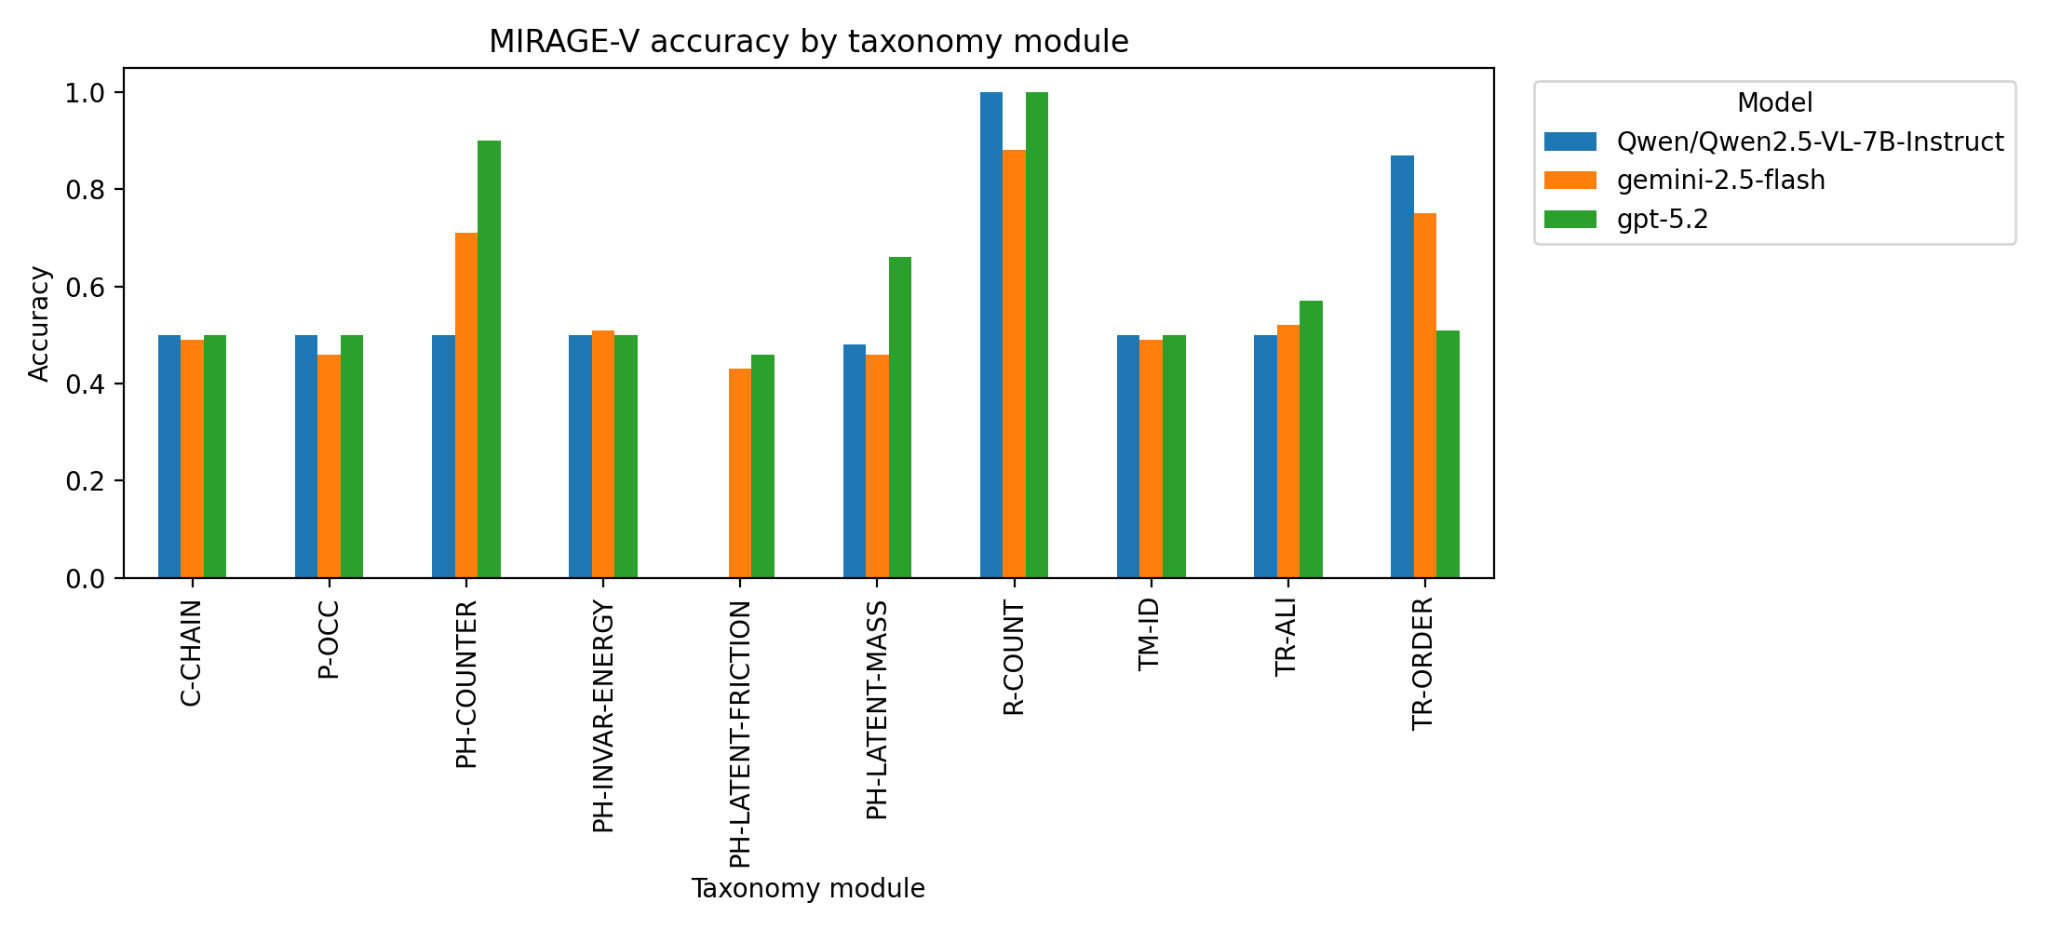
\includegraphics[width=\linewidth]{figures/by_module_accuracy.png}
  \caption{Accuracy by MIRAGE-V taxonomy module for three representative models. All models are evaluated with \FramesPerVideo uniformly sampled frames per video.}
  \label{fig:by-module-accuracy}
\end{figure}

\begin{table}[t]
  \centering
  \small
  \caption{Per-module accuracy (\%, higher is better). Each module contains 100 examples (50 minimal-change pairs).}
  \label{tab:by-module-accuracy}
  % Auto-generated from by_module.csv
\begin{tabular}{lrrr}
\toprule
Module & Qwen2.5-VL-7B & Gemini-2.5-Flash & GPT-5.2 \\
\midrule
C-CHAIN & \textbf{50.0} & 49.0 & \textbf{50.0} \\
P-OCC & \textbf{50.0} & 46.0 & \textbf{50.0} \\
PH-COUNTER & 50.0 & 71.0 & \textbf{90.0} \\
PH-INVAR-ENERGY & 50.0 & \textbf{51.0} & 50.0 \\
PH-LATENT-FRICTION & 0.0 & 43.0 & \textbf{46.0} \\
PH-LATENT-MASS & 48.0 & 46.0 & \textbf{66.0} \\
R-COUNT & \textbf{100.0} & 88.0 & \textbf{100.0} \\
TM-ID & \textbf{50.0} & 49.0 & \textbf{50.0} \\
TR-ALI & 50.0 & 52.0 & \textbf{57.0} \\
TR-ORDER & \textbf{87.0} & 75.0 & 51.0 \\
\bottomrule
\end{tabular}

\end{table}

\subsection{Pair accuracy by taxonomy module}
Pair accuracy is a stricter metric: a pair is correct only if the model answers \emph{both} minimally different videos correctly.
Figure~\ref{fig:by-module-pair-accuracy} and Table~\ref{tab:by-module-pair-accuracy} show that pair accuracy is substantially lower than accuracy for most modules.

\paragraph{Discrimination failures.}
Modules with $\approx$50\% accuracy but near-zero pair accuracy (e.g., C-CHAIN, TM-ID, P-OCC, PH-INVAR-ENERGY for some models) indicate that the model often gives the same answer for both $A$ and $B$ and does not detect the causal intervention.

\paragraph{Sampling sensitivity.}
TR-ALI (micro-teleportation) exhibits low pair accuracy for all models, consistent with sparse sampling missing brief violations.
This motivates MIRAGE-V's critical-window annotations and sparse-vs-dense reporting.

\begin{figure}[t]
  \centering
  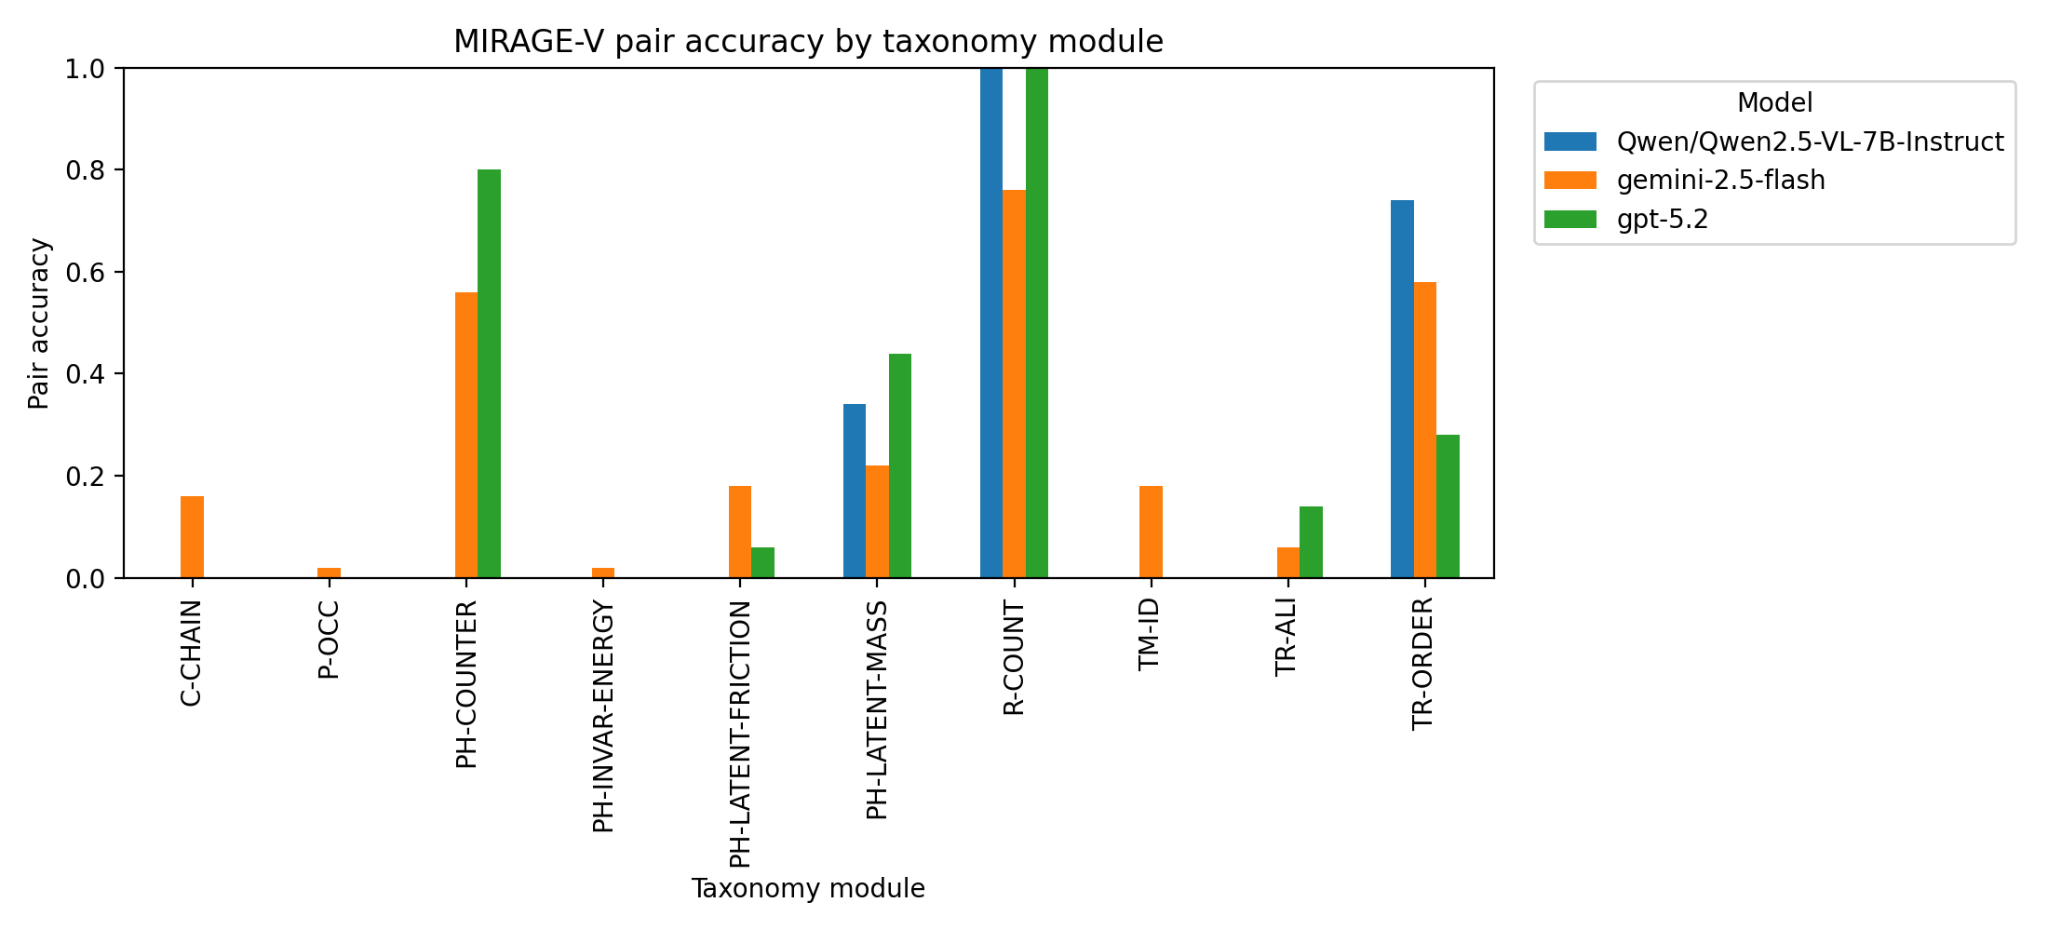
\includegraphics[width=\linewidth]{figures/pair_accuracy_by_module.png}
  \caption{Pair accuracy by taxonomy module. Pair accuracy measures whether a model can discriminate minimal-change pairs rather than relying on priors.}
  \label{fig:by-module-pair-accuracy}
\end{figure}

\begin{table}[t]
  \centering
  \small
  \caption{Per-module pair accuracy (\%, higher is better). Each module contains 50 minimal-change pairs.}
  \label{tab:by-module-pair-accuracy}
  % Auto-generated from pair_accuracy_by_module.csv
\begin{tabular}{lrrr}
\toprule
Module & Qwen2.5-VL-7B & Gemini-2.5-Flash & GPT-5.2 \\
\midrule
C-CHAIN & 0.0 & \textbf{16.0} & 0.0 \\
P-OCC & 0.0 & \textbf{2.0} & 0.0 \\
PH-COUNTER & 0.0 & 56.0 & \textbf{80.0} \\
PH-INVAR-ENERGY & 0.0 & \textbf{2.0} & 0.0 \\
PH-LATENT-FRICTION & 0.0 & \textbf{18.0} & 6.0 \\
PH-LATENT-MASS & 34.0 & 22.0 & \textbf{44.0} \\
R-COUNT & \textbf{100.0} & 76.0 & 100.0 \\
TM-ID & 0.0 & \textbf{18.0} & 0.0 \\
TR-ALI & 0.0 & 6.0 & \textbf{14.0} \\
TR-ORDER & \textbf{74.0} & 58.0 & 28.0 \\
\bottomrule
\end{tabular}
\end{table}

\subsection{Discussion}
Overall, the gap between accuracy and pair accuracy highlights a key evaluation pitfall: moderately high accuracy can arise from biased or shortcut answers, while pair accuracy directly tests whether the model's answer changes appropriately under minimal physical interventions.
MIRAGE-V makes these failure modes explicit through taxonomy labels, critical windows, and mandatory shortcut audits, enabling more actionable diagnosis than aggregate scores alone.
